\documentclass[border=8pt]{standalone}
\usepackage{pgfplots}
\pgfplotsset{compat=1.18}
\begin{document}
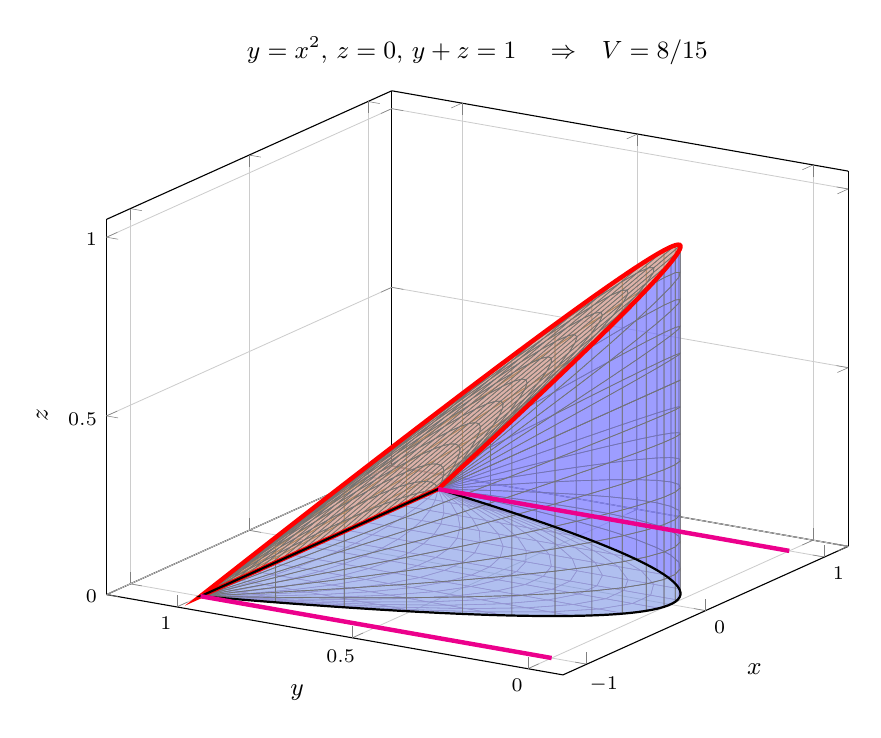
\begin{tikzpicture}
\begin{axis}[
    width=11cm, height=9cm,
    view={-58}{22},
    xlabel={$x$}, ylabel={$y$}, zlabel={$z$},
    xmin=-1.2, xmax=1.2, ymin=-0.1, ymax=1.2, zmin=0, zmax=1.05,
    xtick={-1,0,1}, ytick={0,0.5,1}, ztick={0,0.5,1},
    tick label style={font=\scriptsize},
    label style={font=\small},
    title style={font=\small},
    grid=major, grid style={black!20, line width=0.3pt},
    title={$y=x^{2}$, $z=0$, $y+z=1$ \quad$\Rightarrow$\quad $V=8/15$},
]
\addplot3[surf, domain=-1:1, y domain=0:1, samples=14, samples y=14,
          fill=green!45, fill opacity=0.25, shader=flat,
          draw=black!30, line width=0.2pt]
  ({x}, {x^2 + y*(1-x^2)}, {0});
\addplot3[surf, domain=-1:1, y domain=0:1, samples=22, samples y=14,
          fill=blue!55, fill opacity=0.45, shader=flat,
          draw=black!55, line width=0.25pt]
  ({x}, {x^2}, {y*(1-x^2)});
\addplot3[surf, domain=-1:1, y domain=0:1, samples=22, samples y=14,
          fill=orange!75, fill opacity=0.45, shader=flat,
          draw=black!55, line width=0.25pt]
  ({x}, {x^2 + y*(1-x^2)}, {1-x^2 - y*(1-x^2)});
\addplot3[ultra thick, red, domain=-1:1, samples=60] ({x},{x^2},{1-x^2});
\addplot3[thick, black, domain=-1:1, samples=60] ({x},{x^2},{0});
\addplot3[ultra thick, magenta, domain=0:1, samples=2] ({-1},{x},{0});
\addplot3[ultra thick, magenta, domain=0:1, samples=2] ({1},{x},{0});
\end{axis}
\end{tikzpicture}
\end{document}
